% Requiere en el preambulo: \usepackage{amsmath,graphicx,float}
\section{Fundamentos, muestreo y FFT}\label{sec:fundamentos}
Para comparar las propiedades de la transformada discreta de Fourier (DFT), se utilizaron señales cosenoidales de amplitud unitaria y fase inicial cero, muestreadas a $f_s=8192$ Hz en bloques de $N=1024$ muestras. Todos los resultados se generan con \texttt{pruebas/test\_fft.py}.

\subsection{Relación entre serie de Fourier, transformada de Fourier, DFT y FFT}
Una señal periódica continua de período $T_0$ puede representarse mediante una serie de Fourier, esto es, la suma de componentes armónicas discretas:
\begin{equation}
 x(t)=\sum_{m=-\infty}^{\infty}c_m e^{jm\omega_0 t},\qquad \omega_0=\frac{2\pi}{T_0}.
\end{equation}
Para señales no necesariamente periódicas, la transformada de Fourier describe un espectro continuo:
\begin{equation}
 X(f)=\int_{-\infty}^{\infty}x(t)e^{-j2\pi ft}\,dt.
\end{equation}
Al contar con $N$ muestras de una señal digital, se emplea la DFT, definida por
\begin{equation}
 X[k]=\sum_{n=0}^{N-1}x[n]e^{-j2\pi kn/N},\qquad k=0,\dots,N-1.
\end{equation}
La FFT no constituye una transformada matemática diferente: es una familia de algoritmos para calcular la DFT con menor costo. Frente al cálculo directo de orden $O(N^2)$, una FFT radix-2 para $N$ potencia de dos requiere $O(N\log_2 N)$ operaciones.

\subsection{Separación frecuencial, latencia y memoria}
La separación de bins y la duración de adquisición de un bloque se relacionan mediante
\begin{equation}
 \Delta f=\frac{f_s}{N}=\frac{1}{T},\qquad T=\frac{N}{f_s}.
\end{equation}
Con $f_s=8192$ Hz y $N=1024$ se obtiene $\Delta f=8$ Hz y $T=0.125$ s. Los bins positivos están ubicados en $f_k=k\Delta f$ hasta Nyquist ($4096$ Hz). Como comparación, para $N=512,1024,2048,4096$, las separaciones son $16,8,4,2$ Hz y los tiempos de adquisición son $62.5,125,250,500$ ms, respectivamente. Aumentar $N$ permite un muestreo más denso del espectro, pero exige más memoria y mayor tiempo de adquisición. El tiempo de procesamiento se agrega a esa latencia; el tamaño del bloque por sí solo no determina toda la latencia del sistema. Además, separar dos tonos cercanos depende también de la ventana, el ruido y el ancho de los lóbulos, no solo de $\Delta f$.

\subsection{Tono alineado y tono entre bins: fuga espectral y ventanas}
Se estudiaron las dos señales
\begin{equation}
 x_1[n]=\cos\!\left(2\pi\frac{512}{8192}n\right),\qquad
 x_2[n]=\cos\!\left(2\pi\frac{516}{8192}n\right).
\end{equation}
El primer tono corresponde al bin $k=64$, mientras el segundo se ubica a mitad de camino entre los bins 64 ($512$ Hz) y 65 ($520$ Hz). Antes de la FFT se comparó la ventana rectangular $w_R[n]=1$ con la Hann periódica:
\begin{equation}
 w_H[n]=\frac12\left(1-\cos\left(\frac{2\pi n}{N}\right)\right),\quad 0\le n<N.
\end{equation}
Para mostrar la magnitud de las señales, se normalizaron los valores obtenidos de la FFT tomando en cuenta la ventana utilizada. Además, se ajustaron las componentes de frecuencia cero (DC) y Nyquist para evitar contar su magnitud dos veces.

En las gráficas de fase, solamente se muestran las frecuencias cuya magnitud supera el 1\% del valor máximo. Esto se hizo porque la fase de componentes con magnitudes muy pequeñas no aporta información útil para el análisis.

\begin{figure}[H]
 \centering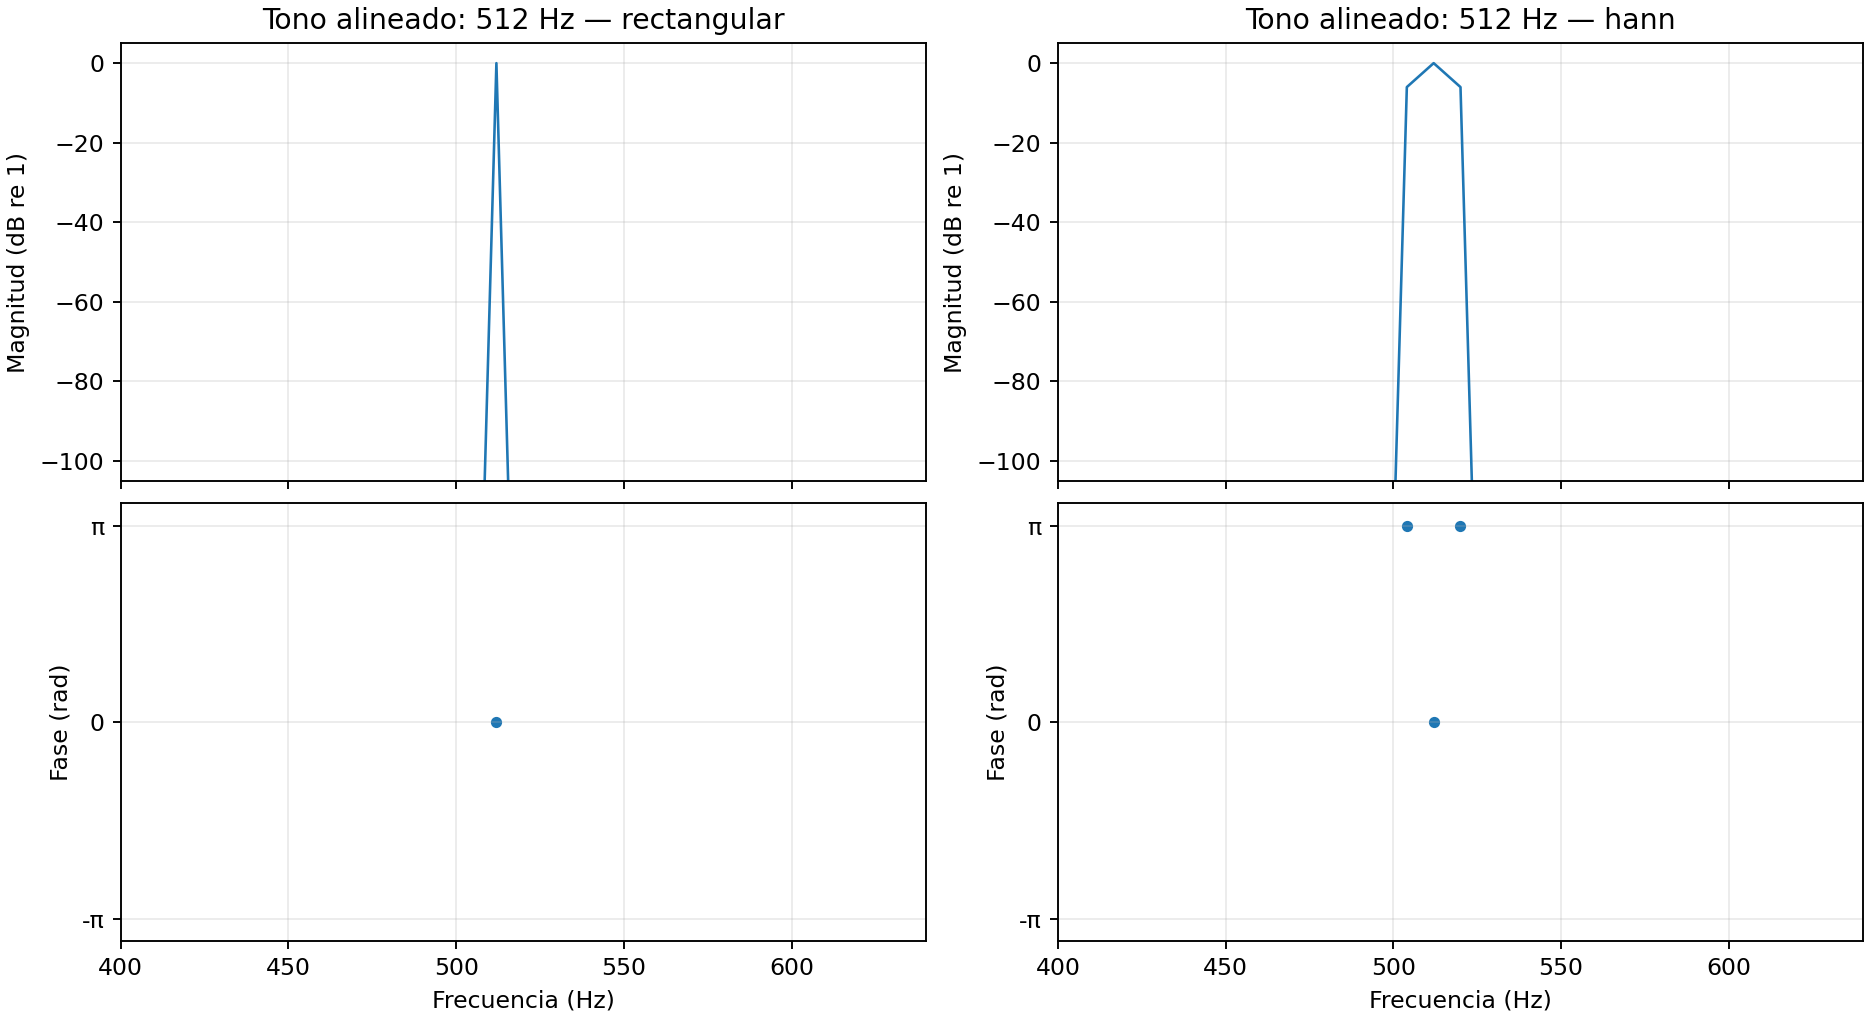
\includegraphics[width=\linewidth]{resultados/figuras/fig_21_bin.png}
 \caption{Magnitud y fase del tono alineado con un bin, comparando ventana rectangular y Hann.}\label{fig:bin}
\end{figure}
\begin{figure}[H]
 \centering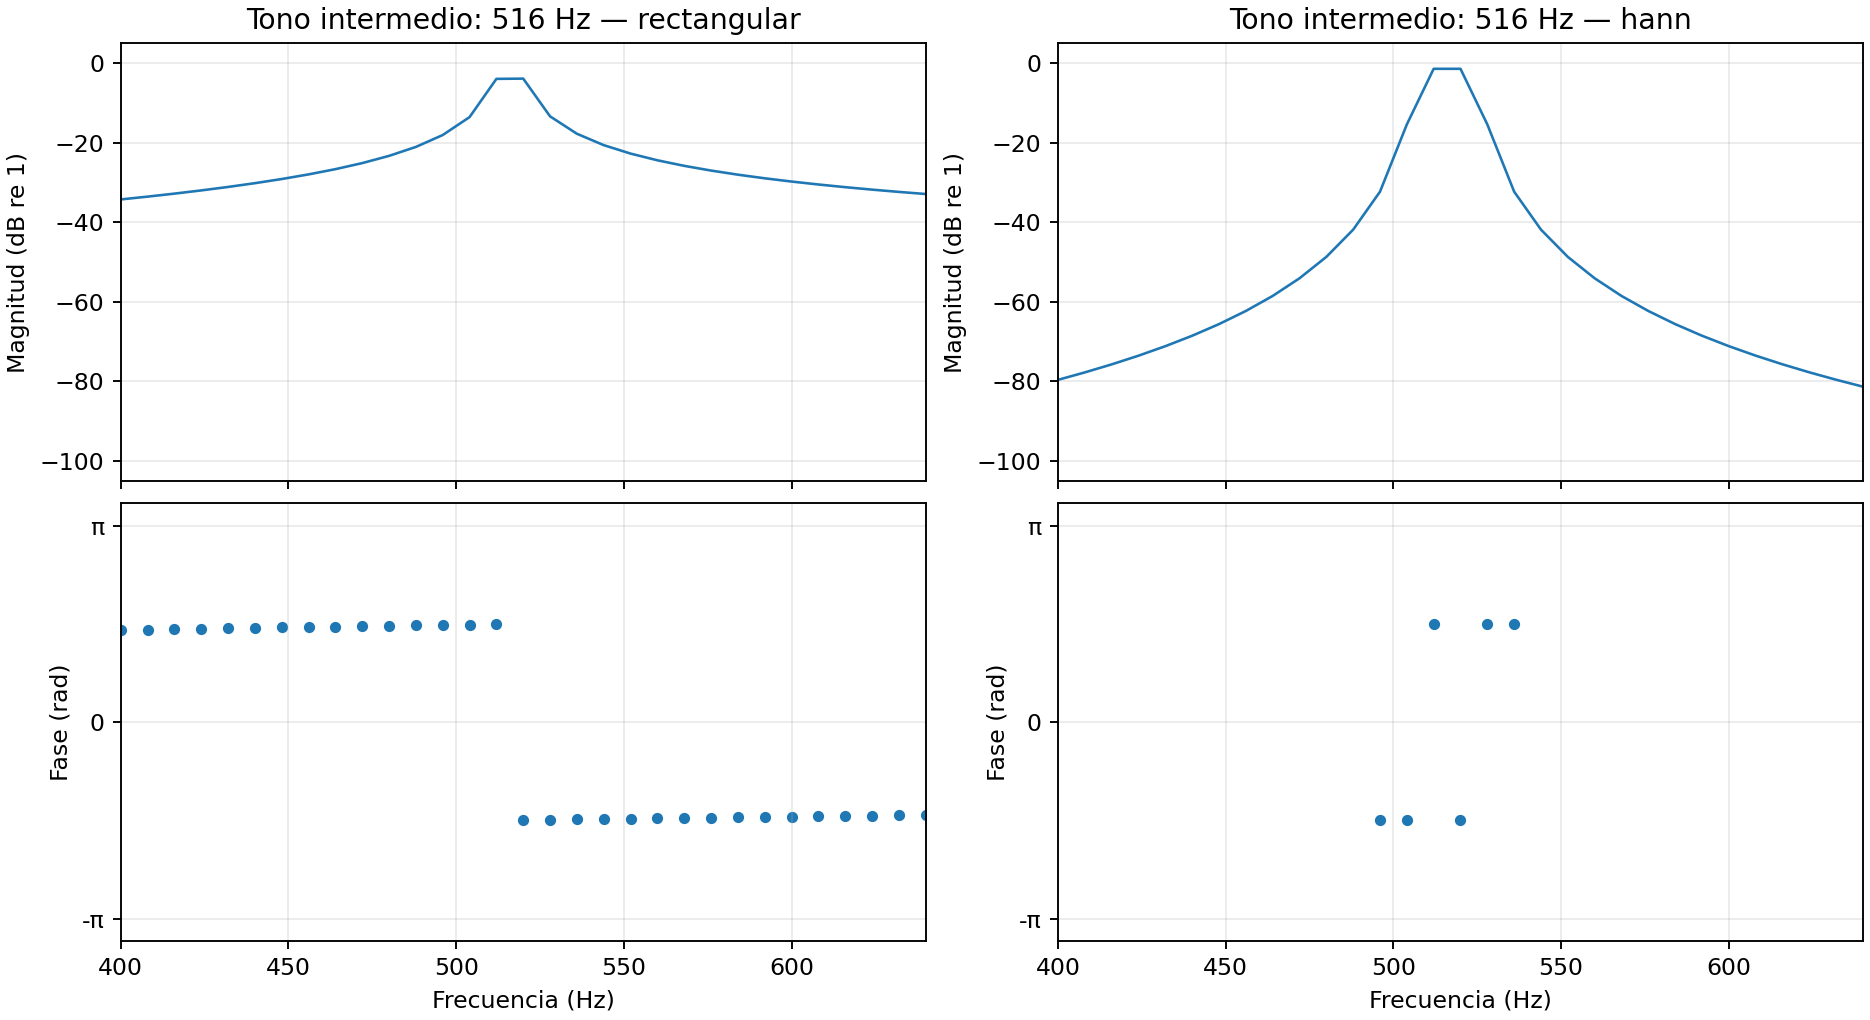
\includegraphics[width=\linewidth]{resultados/figuras/fig_21_entre_bins.png}
 \caption{Magnitud y fase del tono ubicado entre dos bins.}\label{fig:inter}
\end{figure}
Al utilizar la ventana rectangular con el tono de 512 Hz, se observa que la energía se concentra en una sola frecuencia. Con la ventana Hann, la energía se distribuye principalmente entre esa frecuencia y las más cercanas.

Para el tono de 516 Hz, la energía se reparte entre varias frecuencias porque el tono no coincide exactamente con un bin de la DFT. Este efecto se conoce como fuga espectral.

La ventana rectangular concentra mejor la energía alrededor de la frecuencia principal, pero presenta mayor fuga hacia otras frecuencias. Por otro lado, la ventana Hann reduce esta fuga, aunque distribuye la energía en un rango más amplio alrededor del tono.

Por lo tanto, la ventana Hann resulta útil para distinguir señales débiles de otras más fuertes, mientras que la rectangular puede ser más conveniente para separar frecuencias muy cercanas.

\subsection{Simetría conjugada de las señales reales}
Para $x[n]\in\mathbb{R}$, la DFT presenta simetría conjugada:
\begin{equation}
 X[N-k]=X^*[k],\qquad k=1,\dots,N-1.
\end{equation}
Esto implica magnitudes iguales y fases opuestas (módulo $2\pi$) en frecuencias positivas y negativas. Para el tono de 516 Hz, el error máximo medido $\max_{1\le k<N/2}|X[k]-X^*[N-k]|$ fue $3.63\times10^{-14}$. Como comprobación adicional se anularon los bins 63, 64 y 65 y sus correspondientes bins negativos. La parte imaginaria máxima de la IFFT resultante fue $2.64\times10^{-16}$, consistente con un error de redondeo numérico.
\begin{figure}[H]
 \centering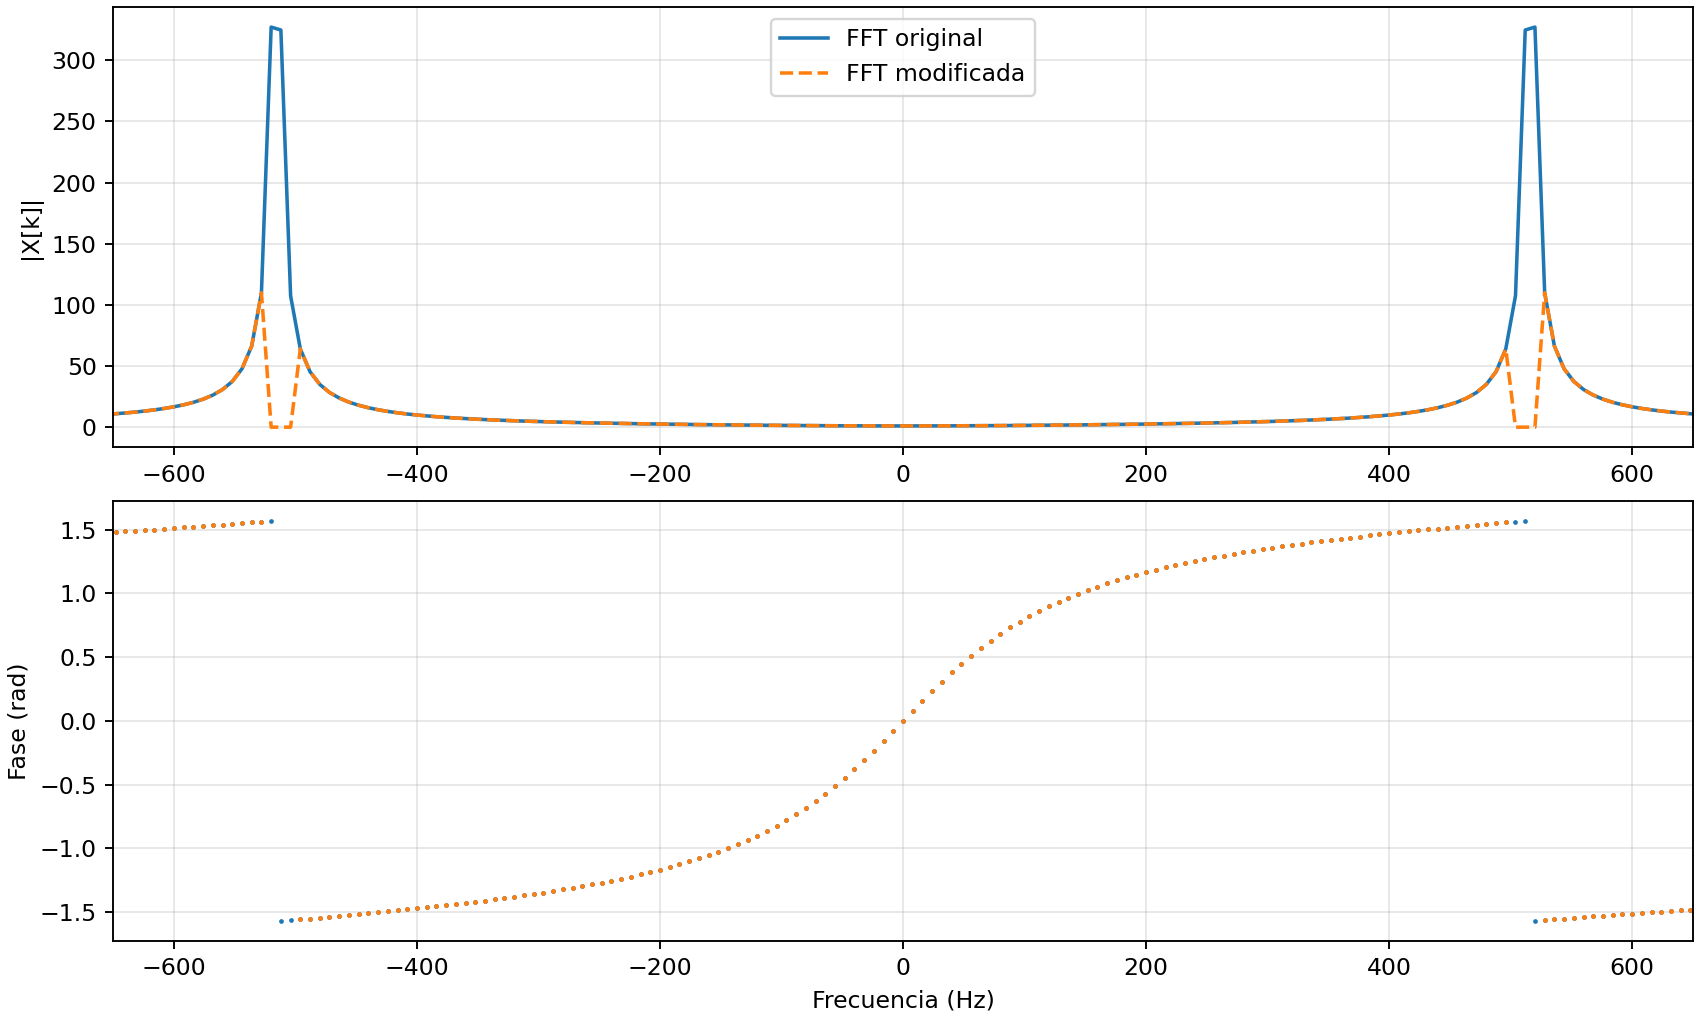
\includegraphics[width=\linewidth]{resultados/figuras/fig_21_simetria.png}
 \caption{Espectro de magnitud y fase antes y después de una modificación conjugadamente simétrica.}\label{fig:simetria}
\end{figure}
La simetría debe mantenerse al alterar el espectro antes de usar la IFFT para que la señal reconstruida siga siendo real. Para índices auto-conjugados, DC ($k=0$) y Nyquist ($k=N/2$ cuando $N$ es par), los coeficientes también deben ser reales.
